\documentclass[12pt,a4paper]{article}
\usepackage[utf8]{inputenc}
\usepackage[english]{babel}
\usepackage{enumerate}
\usepackage{amsmath}
\usepackage{amsfonts}
\usepackage{amssymb}
\usepackage{graphicx}
\usepackage{fourier}
\usepackage[left=2cm,right=2cm,top=2cm,bottom=2cm]{geometry}
\usepackage{commath}
\usepackage{cancel}
\usepackage{placeins}
\author{Juan Carlos Apitz, ID 012523821}
\title{STAT572 - Homework Assignment 5}
\begin{document}

\maketitle

\section*{In-class 6:}

\textbf{Summary}

$\alpha=0.05$ for all exercises.

\begin{figure}[ht!] 
\begin{center}
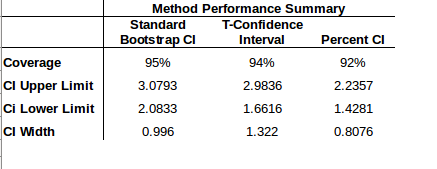
\includegraphics[scale=.7]{inClass_summary.png}
\caption{Performance Summary}
\label{inclass6 fig0}
\end{center}
\end{figure}
\FloatBarrier

\begin{enumerate}[a)]

\item{\textbf{Standard Bootstrap Confidence Interval}\\
\textit{MATLAB Code:}
\begin{verbatim}
% STANDARD BOOTSTRAP CI
counter = 0; B = 500;
meand = 2; stdev = 1;
thetahatb = zeros(1,100);

for i=1:100
    % generate data and calculate stat of interest
    rs = normrnd(meand,stdev,1,20);
    thetahat = median(rs);
    
    % set up the Bootstrap
    bvals = bootstrp(B, @(x) median(x),rs);
    
    % calculate the Bootstrap SE
    seb = std(bvals);
    
    % calculate the CI
    alpha = 0.05;
    cilo = thetahat-norminv(1-alpha/2,0,1)*seb;
    cihi = thetahat-norminv(alpha/2,0,1)*seb;
    if cihi >= 2 && cilo <= 2
        counter = counter + 1;
    end
    thetahatb(i) = mean(bvals);
end
hist(thetahatb)
set(get(gca,'child'),'FaceColor',[.9 .9 .9],'EdgeColor','black');
title('Boostrapped Estimated Median Histogram')
ylabel('Frequency'); xlabel('Estimated Median for each of the 100 runs')
\end{verbatim}

\textit{Results}\\
\begin{verbatim}
>> stdBoot
>> counter

counter =

95
\end{verbatim}

\textit{Histogram}

\begin{figure}[ht!] 
\begin{center}
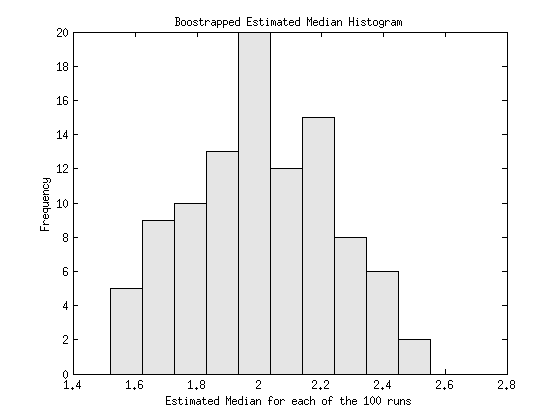
\includegraphics[scale=.7]{inClass_std_hist.png}
\caption{}
\label{inclass6 fig1}
\end{center}
\end{figure}
\FloatBarrier
}

\item{\textbf{Bootstrap t-Confidence Interval}\\
\textit{MATLAB Code:}\\
\begin{verbatim}
% BOOTSTRAP t-CONFIDENCE INTERVAL
counter = 0;
B = 500; thetahatb = zeros(1,100);
meand = 2; stdev = 1;
alpha = 0.05;

for i =1:100
    % generate data and calculate stat of interest
    rs = normrnd(meand,stdev,1,20);
    thetahat = median(rs);
    
    % Get the bootstrap replicates and samples.
    [bootreps, bootsam] = bootstrp(B,@(x) median(x),rs);
    % Set up some storage space for the SEs.
    sehats = zeros(size(bootreps));
    % Each column of bootsam contains indices
    % to a bootstrap sample.
    for j = 1:B
        % extract the sample from the data
        xstar = rs(bootsam(:,j));
        bvals(j) = median(xstar);
        % Do bootstrap using that sample to estimate SE.
        sehats(j) = std(bootstrp(20,@(x) median(x),xstar));
    end
    zvals = (bootreps - thetahat)./sehats;
    
    % Estimate the SE using the bootstrap.
    SE = std(bootreps);
    
    % Get the quantiles.
    k = round(B*alpha/2);
    szval = sort(zvals);
    tlo = szval(k);
    thi = szval(B-k);
    % Get the endpoints of the interval.
    cilo = thetahat-thi*SE;
    cihi = thetahat-tlo*SE;
    if cihi >= 2 && cilo <= 2
        counter = counter + 1;
    end
    thetahatb(i) = mean(bootreps);
end
hist(thetahatb)
set(get(gca,'child'),'FaceColor',[.9 .9 .9],'EdgeColor','black');
title('Boostrapped Estimated Median Histogram')
ylabel('Frequency'); xlabel('Estimated Median for each of the 100 runs')
\end{verbatim}
\textit{Results}\\
\begin{verbatim}
>> tBoot
>> counter
counter =
    94
\end{verbatim}

\textit{Histogram}

\begin{figure}[ht!] 
\begin{center}
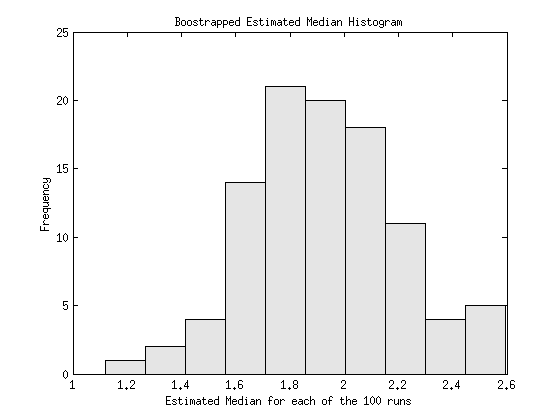
\includegraphics[scale=.7]{inClass_t_hist.png}
\caption{}
\label{inclass6 fig2}
\end{center}
\end{figure}
\FloatBarrier
}

\item{\textbf{Bootstrap  Percentile Confidence Interval}\\
\textit{MATLAB Code:}\\
\begin{verbatim}
% BOOTSTRAP PCT CONFIDENCE INTERVAL
clear; counter = 0;
B = 500; thetahatb = zeros(1,100);
meand = 2; stdev = 1;

for i=1:100
    % generate data and calculate stat of interest
    rs = normrnd(meand,stdev,1,20);
    thetahat = median(rs);
    
    % set up the Bootstrap
    B = 500;
    bvals = bootstrp(B, @(x) median(x),rs);
    
    % calculate the Bootstrap SE
    seb = std(bvals);
    
    % find the bootstrap percentile interval
    alpha = 0.05;
    k = round(B*alpha/2);
    thetab = sort(bvals);
    blo = thetab(k);
    bhi = thetab(B-k);
    if bhi >= 2 && blo <= 2
        counter =counter + 1;
    end
    thetahatb(i) = mean(bvals);
end
hist(thetahatb)
set(get(gca,'child'),'FaceColor',[.9 .9 .9],'EdgeColor','black');
title('Boostrapped Estimated Median Histogram')
ylabel('Frequency'); xlabel('Estimated Median for each of the 100 runs')
\end{verbatim}


\textit{Results}\\
\begin{verbatim}
>> pctBoot
>> counter

counter =

    92

>> 
\end{verbatim}

\textit{Histogram}

\begin{figure}[ht!] 
\begin{center}
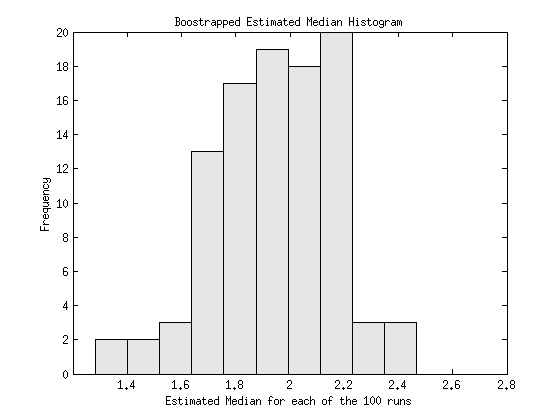
\includegraphics[scale=.7]{inClass_pct_hist.png}
\caption{}
\label{inclass6 fig3}
\end{center}
\end{figure}
\FloatBarrier


}
\end{enumerate}

\clearpage

\section*{Exercise 7.8}
\textit{MATLAB Code:}\\

\begin{verbatim}
% Code for exercise 7.8

% get the dataset
load forearm;
% PART A
n = length(forearm); % sample size
B = 10000;	% number of bootstrap replicates
% Get the value of the statistic of interest.
thetahat = var(forearm,1);

% Use unidrnd to get the indices to the resamples.
inds = unidrnd(n,n,B);
% Extract these from the data.
foreboot = forearm(inds);
thetahatb = var(foreboot,1); % get the 2nd moment for each column using
seb = std(thetahatb);

% PART B
% find the bootstrap percentile interval for the central 2nd moment
% calculate the CI
alpha = 0.05;
cilo = thetahat-norminv(1-alpha/2,0,1)*seb;
cihi = thetahat-norminv(alpha/2,0,1)*seb;

fprintf('Pct Interval for 2nd Central Moment (%2.3f, %3.3f)\n',cilo,cihi)
\end{verbatim}

\textit{Results}

\begin{verbatim}
>> q7p8
Standard Interval for 2nd Central Moment (0.991, 1.502)
>> 
\end{verbatim}

\textit{Discussion}

In this exercise we implement a non-parametric bootstrap estimation of a confidence interval for the second central moment, $\hat{\theta}=\dfrac{1}{n}\sum_{i=1}^n(x_i-\bar{x})^2$. Running the above code we obtain a $95\%$ confidence interval for $\hat{\theta}$ of $(0.991, 1.502)$ (witdh=0.511). Example 7.11 in the class textbook implements the Bootstrap-t confidence interval and obtains $(1.00, 1.57)$, (width=0.57). Example 7.12 implements the Bootstrap-t confidence interval and obtains $(1.03,1.45)$, (with=0.42). Finally, in problem a parametric Bootstrap method is used assuming a normal distribution of the the forearm data. My implementation of this exercise obtains $(1.009,1.499)$, (with=0.49). The smaller width is given by the percentile method, which is also the case for the in-class exercise. A tighter interval might be desirable, however one must be careful not to sacrifice coverage (see in-class results above).

\clearpage

\section*{Exercise 7.9}
\textit{MATLAB Code:}\\

\begin{verbatim}
% Code for exercise 7.9

% get the dataset
load forearm;
% PART A
n = length(forearm); % sample size
B = 10000;	% number of bootstrap replicates
% Get the value of the statistic of interest.
thetahat = mean(forearm);

% Use unidrnd to get the indices to the resamples.
inds = unidrnd(n,n,B);
% Extract these from the data.
foreboot = forearm(inds);
thetahatb = mean(foreboot); % get the mean for each column using
seb = std(thetahatb);

% PART B
% find the bootstrap percentile interval for the central 2nd moment
% calculate the CI
alpha = 0.05;
cilo = thetahat-norminv(1-alpha/2,0,1)*seb;
cihi = thetahat-norminv(alpha/2,0,1)*seb;

% theoretical CI
tcilo = thetahat-norminv(1-alpha/2,0,1)*(std(forearm)/sqrt(n));
tcihi = thetahat-norminv(alpha/2,0,1)*(std(forearm)/sqrt(n));

fprintf('Standard Bootstrap Interval for the mean (%2.3f, %3.3f)\n',cilo,cihi)
fprintf('Theoretical Interval for the mean (%2.3f, %3.3f)\n',tcilo,tcihi)
\end{verbatim}

\textit{Results/Discussion}

For this exercise we implement the algorithm in exercise 7.9 but calculate the 95\% confidence interval for the sample mean, $\bar{x}$ and compare with the theoretical results, shown below:\\

\begin{itemize}

\item{Standard Interval for the mean (18.616, 18.989)}
\item{Theoretical Standard Interval for the mean (18.617, 18.988)}

\end{itemize}

The theoretical results are based on the following calculation: $\biggr(\bar{x}-z_{(0.975)}\dfrac{s}{\sqrt{140}},\bar{x}-z_{(0.025)}\dfrac{s}{\sqrt{140}}\biggr)$.\\

The results seem to indicate that there is close agreement between the bootstrap estimation of the confidence interval and the expected theoretical results; they are very close.


\end{document}